\documentclass[11pt,a4paper,sans]{moderncv}
\usepackage{hyphenat}
\usepackage{lmodern}
\usepackage{silence}
\WarningFilter{latex}{Command \showhyphens}


% ModernCV themes
\moderncvstyle{banking} % style options: 'casual' (default), 'classic', 'oldstyle', 'banking'
\moderncvcolor{blue}    % color options: 'blue' (default), 'orange', 'green', 'red', 'purple', 'grey', 'black'

% Character encoding
\usepackage[utf8]{inputenc}
\usepackage[scale=0.9]{geometry}




% === PERSONAL INFO ===
% Personal data
\firstname{}
\familyname{Pratik Jadhav}
\title{ Programmer | \texorpdfstring{\\}{ }
GATE CSE Qualified} 
\email{pratikjadhav.52239@gmail.com}
\phone[mobile]{+91 7757024513}
\social[linkedin]{linkedin.com/in/pratik-jadhav}
\social[github]{github.com/pratikjadhav2000}
\address{Ramnagar, Pawar Colony}{Satara, Maharashtra}{India}

\begin{document}

 

\begin{flushright}
    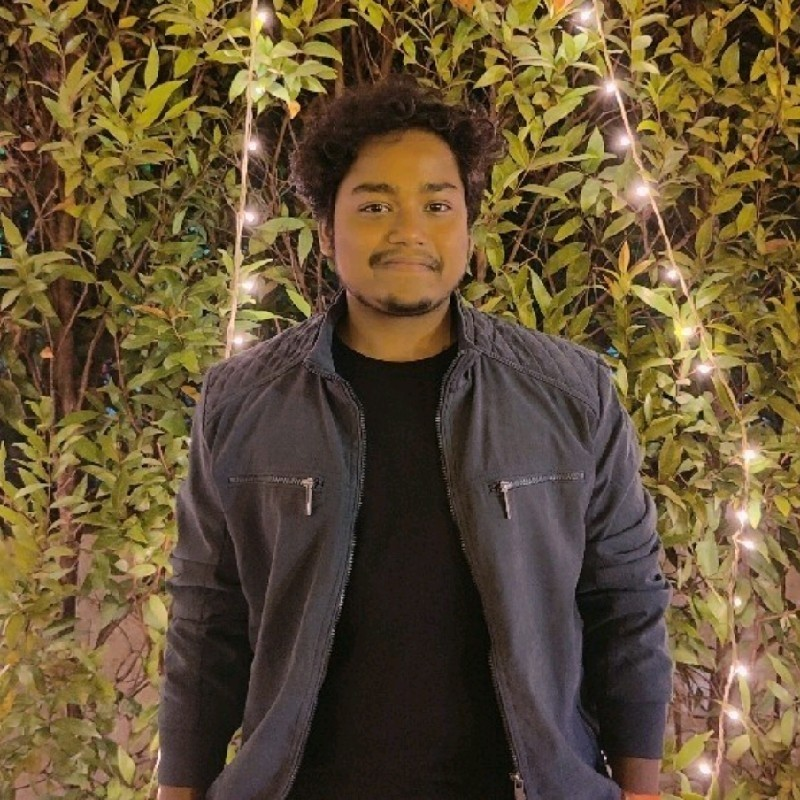
\includegraphics[width=0.13\textwidth]{profilepic.jpg}
\end{flushright}
\vspace{-8.0cm}
 
\vspace{5cm}

\includegraphics[width=0.13\textwidth]{NITLOGO.png}
\vspace{-2.5cm}

    



\makecvtitle

% EXPERIENCE
\section{Experience}
\cventry{Jun 2023 -- Oct 2023}{Senior Software Engineer}{Persistent Systems Ltd}{Pune}{}{
\begin{itemize}
    \item Impact analysis of CRs from client
    \item Feature Development and Deployments
    \item Solving Bugs on QA/UAT/Production
    \item Giving KT sessions on critical builds
    \item Grooming junior team members
\end{itemize}}
\cventry{Jun 2021 -- Jun 2023}{Software Engineer}{Persistent Systems Ltd}{Pune}{}{}
\cventry{Sept 2020 -- Dec 2020}{Software Developer Intern}{BloomIndia}{Bangalore}{}{
\begin{itemize}
    \item Worked as Backend Web Developer in PHP
\end{itemize}}

% EDUCATION
\section{Education}
\cventry{2017 -- 2021}{B.E. in Computer Science and Engineering}{MMCOE, SPPU}{Pune}{}{CGPA: 7.87/10}
\cventry{2017}{HSC (Science)}{Maharashtra Board}{}{66.92\%}{}
\cventry{2015}{SSC}{Maharashtra Board}{}{89.60\%}{}
\cvitem{}{No. of Dead Backlogs – 0}

% CERTIFICATIONS
\section{Certifications}
\cvitem{}{Algorithmic Toolbox - UC San Diego (Coursera)}
\cvitem{}{Data Structures - UC San Diego (Coursera)}
\cvitem{}{Introduction to Git and GitHub - Google (Coursera)}

% SKILLS
\section{Skills}
\cvitem{Programming}{C, C++, Java, PHP}
\cvitem{Concepts}{Algorithms \& Data Structures, OOPS, REST API}
\cvitem{Database}{MySQL}
\cvitem{Tools}{Git, BitBucket, Jenkins, Jira, VSCode, Postman, Workbench}

% ACTIVITY
\section{Activities}
\cvitem{}{Cyber Safety Awareness presentations under Earn and Learn activity by Quick Heal Technologies (Maharashtra Cyber Cell).}
\cvitem{}{Participation in Salesforce Hackathon.}

\newpage
% COURSES
\section{Additional Learning}
\cvitem{}{The Design of the UNIX Operating System (AstroMediComp)}
\cvitem{}{Windows Development - Win32SDK (AstroMediComp)}

% HOBBIES
\section{Hobbies}
\cvitem{}{Solving Rubik’s cube, Table Tennis, Chess, Swimming, Playing Classical Tabla}

% LANGUAGES
\section{Languages}
\cvitem{}{English, Hindi, Marathi}



\end{document}
